\chapter{Anexo}\label{int}
\thispagestyle{fancy}


\section*{Anexo}
En este anexo explicaré brevemente como usar mi proyecto para medir la calidad del aire.Asi como las tecnologias usadas para llevar a cabo el proyecto de fin de grado.
\subsection{Tecnologías:}
\begin{enumerate}
    \item Django: Es un framework web de código abierto escrito en Python que permite el desarrollo rápido y eficiente de aplicaciones web.
    \item Bot en Telegram: Se utiliza para la interacción con el usuario.
    \item OpenCv: Es una librería de visión por computadora de código abierto escrita en C++ y Python, se utiliza en este proyecto para desarrollar un script capaz de detectar puntos en una imagen.
    \item Python Es un lenguaje de programación de alto nivel, interpretado y multiplataforma.
    \item SQLite: Base de datos usada para alojar la informacion relevante a la contaminación.
    \item LaTex : Para la redacción de la memoria
    \item Github: Es una forja para alojar proyectos utilizando el sistema de control de versiones Git.
\end{enumerate}
\subsection{Manual de uso :}
Lo primero que deberíamos de hacer será clonar el \hyperlink{https://github.com/aitormorais/TrabajoFinGrado}{repositorio} de GitHub con el siguiente comando:
\begin{lstlisting}[ caption=clonar repositorio ]
git clone https://github.com/aitormorais/TrabajoFinGrado
\end{lstlisting}
una vez este proceso se ha completado tendrás que instalar todas las dependencias con el siguiente comando:
 \begin{lstlisting}[ caption=instalar instalar todas las dependencias ]
pip install -r requirements.txt
\end{lstlisting} una vez las dependencias han sido instaladas será necesario tener dos terminales activas, y ejecutar en cada una de ellas el siguiente comando:
\begin{lstlisting}[ caption=arrancar web terminal 1 ]
python manage.py runserver
\end{lstlisting}
\begin{lstlisting}[ caption=arrancar bot ]
python bot.py
\end{lstlisting}

\begin{figure}[H]
\centering
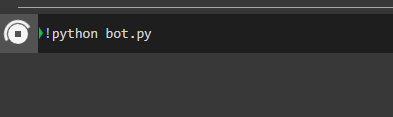
\includegraphics[scale=1]{imgs/lanzar.png}
\end{figure}

Accede a la aplicación de Telegram, es importante usarla desde el móvil, ya que por ahora no es posible mandar la ubicación desde el ordenador.Busca el siguiente nombre: 
\begin{figure}[h]
\centering

\includegraphics[scale=1]{imgs/bot.png}
\end{figure} \\
una vez estés en el bot introduce la ubicación clicando el clip y después dándole a ubicación, seguido añade la foto donde se encuentra plasmada la contaminación, acto seguido accede a la web y verás la actualización en el mapa
\begin{figure}[H]
\centering
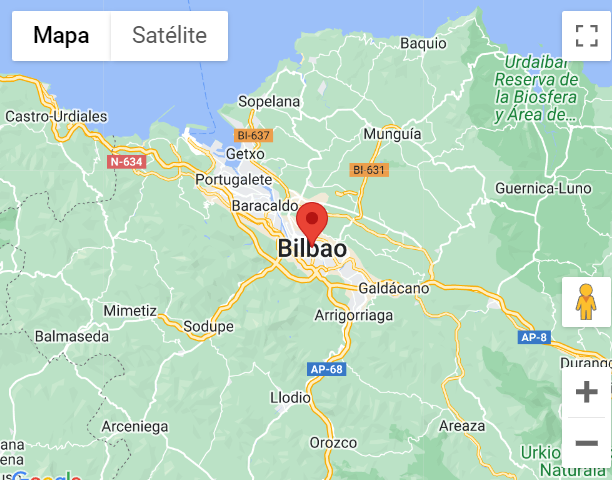
\includegraphics[scale=1]{imgs/map.png}
\end{figure}









